\section{Synthetic Benchmarks with Optimal Teachers}
\label{sec:synthetic}

We begin with controlled synthetic tasks where teacher quality is not a variable---the teacher is always optimal.
This isolates how different memory mechanisms interact with distillation.

\paragraph{T-Maze (retention).}

\begin{table}[ht]
\centering
\caption{T-Maze accuracy ($\uparrow$, max${=}1.0$) across corridor lengths. Optimal teacher, 1000 demos, 3 seeds.}
\label{tab:tmaze}
\begin{tabular}{lcccc}
\toprule
Architecture & $L=10$ & $L=50$ & $L=100$ & $L=200$ \\
\midrule
GRU            & $1.00 \pm .00$ & $1.00 \pm .00$ & $1.00 \pm .00$ & $\mathbf{1.00 \pm .00}$ \\
LSTM           & $1.00 \pm .00$ & $1.00 \pm .00$ & $1.00 \pm .00$ & $\mathbf{1.00 \pm .00}$ \\
Transformer    & $1.00 \pm .00$ & $1.00 \pm .00$ & $1.00 \pm .00$ & $0.05 \pm .02$ \\
STU-T          & $0.05 \pm .02$ & $0.05 \pm .02$ & $0.05 \pm .02$ & $0.05 \pm .02$ \\
\bottomrule
\end{tabular}
\end{table}

GRU and LSTM achieve perfect accuracy on corridors up to 200 steps---0 failures across 3 seeds each (\cref{tab:tmaze}).
Transformer succeeds up to $L{=}100$ but fails at $L{=}200$: its 64-step sliding window cannot reach the hint at step~0, a structural limitation that no amount of training data can fix.
STU-T (the tensordot approximation) fails at every corridor length, a catastrophic failure we analyze below.
With an optimal teacher and sufficient demonstrations, retention is trivially solved by any recurrent architecture---the gating mechanisms configure to preserve the hint signal without difficulty.

\paragraph{CopyTask (recall).}

\begin{table}[ht]
\centering
\caption{CopyTask: mean return ($\uparrow$, max${=}N$). 1000 demos, 3 seeds.}
\label{tab:copy-standard}
\begin{tabular}{lccc}
\toprule
Architecture & $N=5$ & $N=10$ & $N=20$ \\
\midrule
Transformer    & $3.87 \pm 0.09$ & $\mathbf{8.98 \pm 0.01}$ & $\mathbf{18.84 \pm 0.04}$ \\
GRU            & $\mathbf{4.00 \pm 0.00}$ & $\mathbf{9.00 \pm 0.00}$ & $13.60 \pm 0.57$ \\
LSTM           & $\mathbf{4.00 \pm 0.00}$ & $8.33 \pm 0.48$ & $9.78 \pm 0.38$ \\
STU-T          & $\mathbf{4.00 \pm 0.00}$ & $1.09 \pm 0.03$ & $2.31 \pm 0.07$ \\
\bottomrule
\end{tabular}
\end{table}

CopyTask reveals where architecture \emph{does} matter.
At $N{=}20$, Transformer achieves $18.84/20$ (94\%) while GRU reaches only $13.60$ (68\%) and LSTM $9.78$ (49\%).
The mechanism is structural: during recall, the Transformer directly attends to stored tokens via content-addressable lookup, bypassing the information bottleneck of a fixed-size hidden state~\citep{chen2021decision}.
This refines the picture: architecture-independence holds for \emph{retention} but not for \emph{recall}.
The relevant axis is memory mechanism, not inductive bias.

\paragraph{Data efficiency.}
On CopyTask ($N{=}10$), no architecture (excluding STU-T) shows a consistent data efficiency advantage across demonstration budgets from 5 to 1{,}000 (\cref{fig:synthetic-summary}c).
All follow similar trajectories, with Transformer pulling ahead only above 250 demonstrations due to its recall advantage.
On T-Maze ($L{=}100$), GRU achieves perfect accuracy from just 5 demonstrations, while LSTM requires 10---the only condition where architecture matters with an optimal teacher.
Adding a JEPA auxiliary loss~\citep{assran2023ijepa, lecun2022path} recovers LSTM to $1.00$ at budget${=}5$, but this is the only condition where JEPA provides a measurable benefit; across all other architectures, budgets, and tasks, JEPA shows no consistent effect (\cref{fig:jepa-null}; we note that the self-supervised JEPA sweep was conducted on STU-T, which fails independently; the teacher-supervised null on GRU, LSTM, and Transformer is the more informative result).

\begin{figure}[ht]
\centering
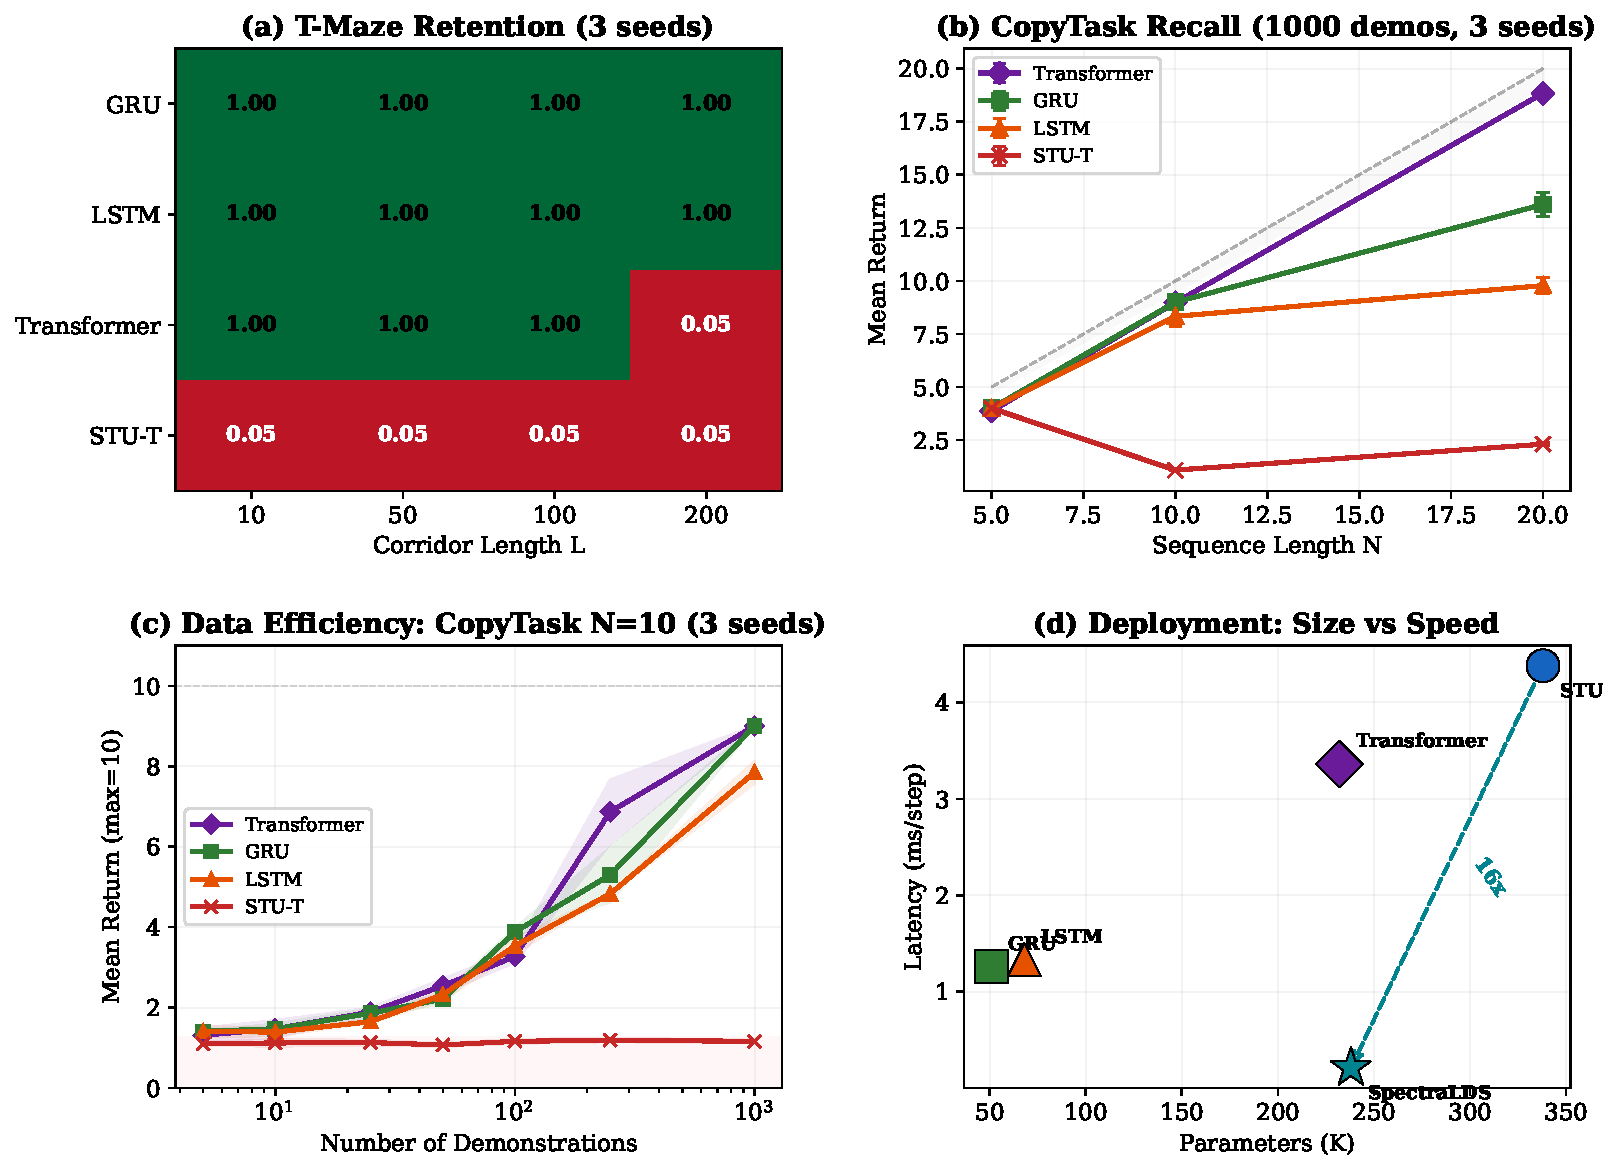
\includegraphics[width=\textwidth]{FIGURE_1_main_4panel.pdf}
\caption{\textbf{Synthetic benchmark summary.} (a)~T-Maze retention: GRU and LSTM hold the hint perfectly; Transformer fails at $L{=}200$ (window exceeded); STU-T fails everywhere. (b)~CopyTask recall: Transformer pulls away at $N{=}20$ via content-addressable lookup. (c)~Data efficiency on CopyTask $N{=}10$: all viable architectures follow similar trajectories; Transformer separates above 250 demos. (d)~Deployment trade-off: GRU and LSTM are Pareto-optimal for latency; SpectraLDS conversion yields $16\times$ speedup over full STU.}
\label{fig:synthetic-summary}
\end{figure}

\begin{figure}[ht]
\centering
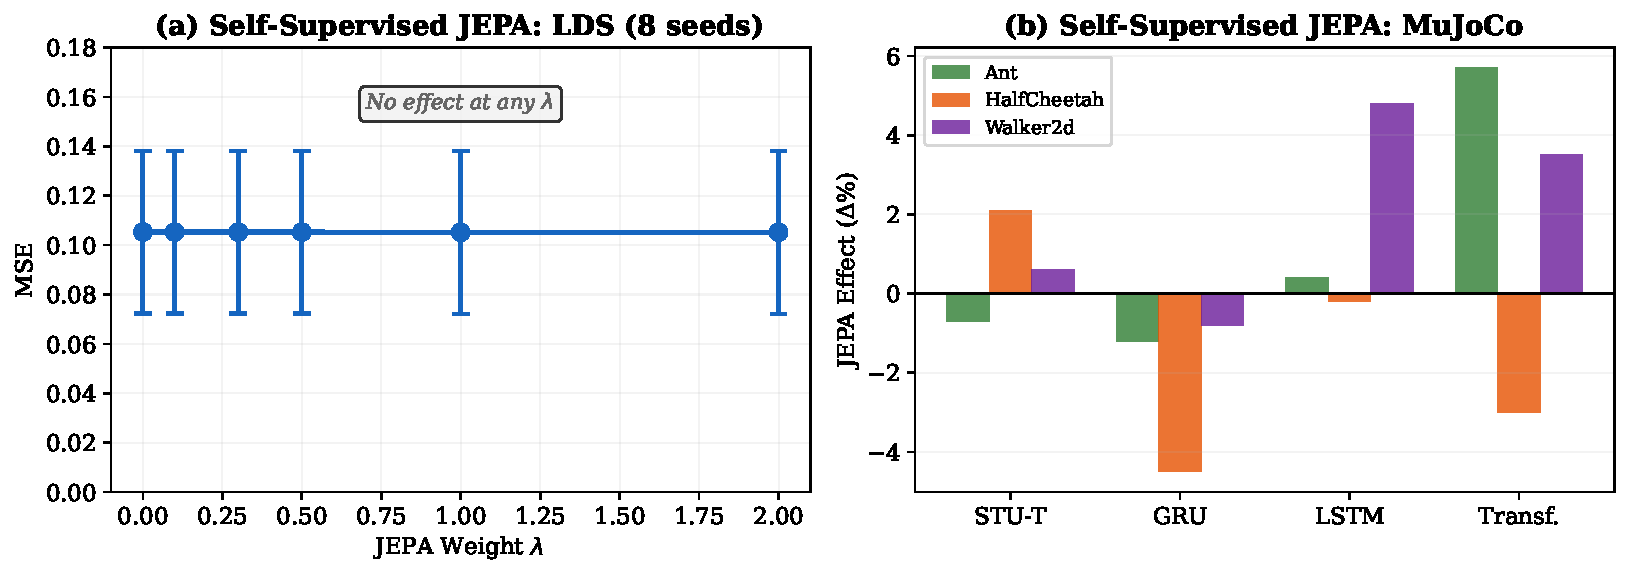
\includegraphics[width=\textwidth]{FIGURE_2_jepa_null_2panel.pdf}
\caption{\textbf{JEPA auxiliary loss produces no consistent benefit.} (a)~Self-supervised JEPA on LDS: MSE is flat at $0.105$ across all $\lambda$ values (8 seeds). (b)~Self-supervised JEPA on MuJoCo: per-architecture effect ranges from $-4.5\%$ to $+5.7\%$ with no consistent direction.}
\label{fig:jepa-null}
\end{figure}

\paragraph{STU-T tensordot failure.}
\label{sec:stu-t-failure}

\begin{table}[ht]
\centering
\caption{Flash STU LDS replication: MSE ($\downarrow$). 16 seeds. Full STU achieves substantially lower MSE (up to $40\times$ vs LSTM) than all other architectures. STU-T tensordot is worst despite using identical spectral filters.}
\label{tab:lds-replication}
\begin{tabular}{lcccc}
\toprule
Model & $\rho=0.9$ & $\rho=0.95$ & $\rho=0.99$ & $\rho=0.999$ \\
\midrule
STU (full)  & $\mathbf{.0003}$ & $\mathbf{.0004}$ & $\mathbf{.0004}$ & $\mathbf{.0003}$ \\
GRU         & $.002$ & $.002$ & $.005$ & $.008$ \\
LSTM        & $.002$ & $.002$ & $.007$ & $.012$ \\
Transformer & $.014$ & $.023$ & $.046$ & $.062$ \\
STU-T       & $.054$ & $.072$ & $.104$ & $.121$ \\
\bottomrule
\end{tabular}
\end{table}

Our STU and STU-T implementations follow the architecture described in~\citet{agarwal2024spectral} and~\citet{liu2025flashstu}, using their published hyperparameters ($K{=}16$ filters, same learning rate and optimizer) without additional tuning at our compact scale; we verified our full STU reproduces their published LDS results at $d_\text{model}{=}64$ (\cref{tab:lds-replication}).
The Flash STU tensordot approximation factorizes each filter's projection matrix $M_k \approx M^{(1)} \otimes M^{(2)}$, reducing parameters from $2K \cdot d^2$ to $2K \cdot d + d^2$.
At the Flash STU paper's scale ($d_\text{model} \geq 128$, 4+ layers), this is tight.
At our compact student scale ($d_\text{model}=64$, 2 layers), the rank-1 Kronecker constraint is catastrophic: STU-T achieves $0.104$ MSE on LDS at $\rho{=}0.99$, compared to $0.002$ published by~\citet{liu2025flashstu} at $d_\text{model}{=}128$---a $52\times$ gap, though we note the comparison is across different model scales.
Against our own full STU at the \emph{same} $d_\text{model}{=}64$, STU-T is $260\times$ worse ($0.104$ vs $0.0004$), isolating the tensordot factorization as the cause.
On all distillation tasks beyond the easiest condition (CopyTask $N{=}5$, where every architecture achieves perfect scores), STU-T scores at chance level.
Meanwhile, full STU achieves the best sequence prediction of any architecture ($5$--$27\times$ lower MSE than GRU on LDS, depending on spectral radius), confirming the spectral prior is powerful---the tensordot approximation destroys it at compact scale.
This finding is unreported in prior work~\citep{liu2025flashstu, agarwal2024spectral} and directly relevant to practitioners building compact spectral models.

\begin{figure}[ht]
\centering
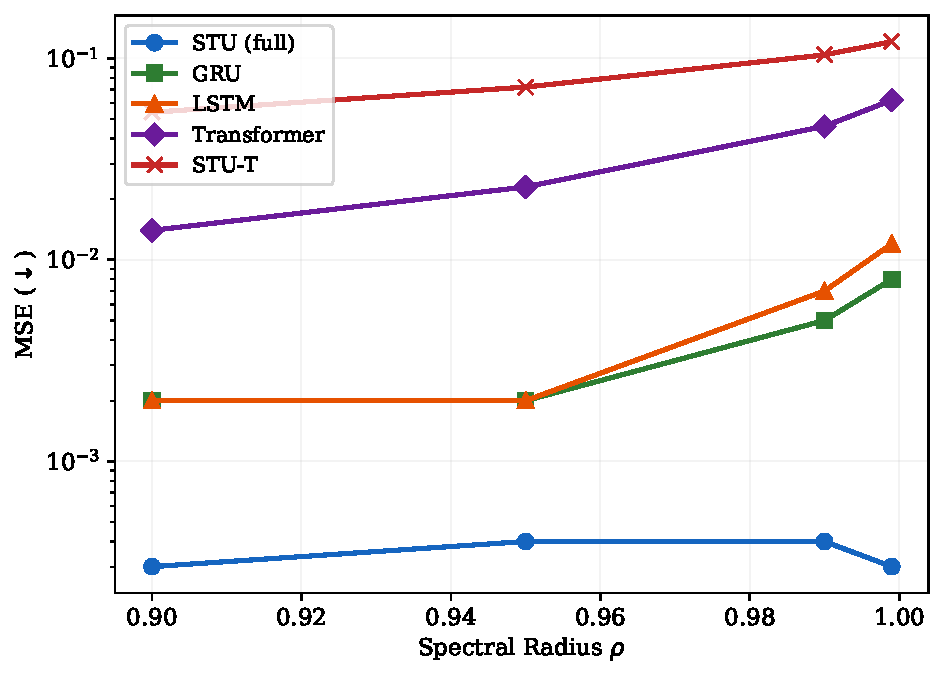
\includegraphics[width=0.5\textwidth]{FIGURE_3_lds_replication.pdf}
\caption{LDS replication (16 seeds, log scale). Full STU achieves $0.0003$ MSE. STU-T is worst at every spectral radius despite using the same spectral filters.}
\label{fig:lds-replication}
\end{figure}
\vspace{-6pt}

With optimal teachers, the synthetic benchmarks establish three points: (1) retention is trivially solved by recurrent models, (2) recall requires attention, and (3) the STU-T tensordot approximation fails catastrophically at compact scale.
The critical question is whether these patterns hold when teachers are imperfect.
